\documentclass[12pt,english]{article}
\usepackage{mathptmx}

\usepackage{color}
\usepackage[dvipsnames]{xcolor}
\definecolor{darkblue}{RGB}{0.,0.,139.}

\usepackage[top=1in, bottom=1in, left=1in, right=1in]{geometry}

\usepackage{amsmath}
\usepackage{amstext}
\usepackage{amssymb}
\usepackage{setspace}
\usepackage{lipsum}

\usepackage[authoryear]{natbib}
\usepackage{url}
\usepackage{booktabs}
\usepackage[flushleft]{threeparttable}
\usepackage{graphicx}
\usepackage[english]{babel}
\usepackage{pdflscape}
\usepackage[unicode=true,pdfusetitle,
 bookmarks=true,bookmarksnumbered=false,bookmarksopen=false,
 breaklinks=true,pdfborder={0 0 0},backref=false,
 colorlinks,citecolor=black,filecolor=black,
 linkcolor=black,urlcolor=black]
 {hyperref}
\usepackage[all]{hypcap} % Links point to top of image, builds on hyperref

\linespread{2}

\begin{document}

\begin{singlespace}
\title{Determinants of Victory in the National Football League\thanks{Acknowledgements here, if any.}}
\end{singlespace}

\author{Alexandra Penner\thanks{Department of Economics, University of Oklahoma.\
E-mail~address:~\href{mailto:alexandra.penner@ou.edu}{alexandra.penner@ou.edu}}}

% \date{\today}
\date{May 8, 2018}

\maketitle

\begin{abstract}
\begin{singlespace}
This project looks at various statistics used to evaluate the performance of NFL teams, using logistic regression to identify the most measures most predictive of a Team winning a game.  This have implications in NFL personnel management, and sports journalism.
\end{singlespace}

\end{abstract}
\vfill{}


\pagebreak{}



\section{Introduction}
Traditionally, Football fans and sports journalists have focused on volume statistics to evaluate team quality, such as total yards, and time of possession, along side a limited number of efficiency stats, specifically passing completion percentage and yards per play.  The newer generation of more data driven journalism on blogs such as Fivethirtyeight, and SB Nation reject a volume statistics approach all together and focus only on efficiency statistics and other advanced stats.  This paper will compare those statistical approaches to identify which stats are most predictive of victory.  The implications of this research are primarily in the improvement of football journalism, as better knowledge of the significance and magnitude of common football stats will allow for better informed writing, and better prioritization of information on sports apps and websites. Additionally this may have implications for the College Football Playoff Committee

The expected outcome of this analysis is a confirmation of the advanced stats approach.  I anticipate that that efficiency statistics, turnovers, and field position will be most predictive of winning, while volume statistics will be less predictive.  For statistics other than turnovers and penalties I would expect a positive relationship with the probability of winning.  While, I would expect that penalty yards and turnovers will be inversely related to probability of winning.  

\section{Literature review}
SB Nation's Football Study Hall publishes a weekly Five Factors Box Score of the five statistics in college football which they find to be the most highly correlated with winning.  These factors are explosiveness, efficiency, field position, finishing drives, and turnovers\footnote{\citet{Con14}}. Explosiveness is how commonly does a team make big plays, Football Study hall uses Equivalent Points per Play, or PPP to measure explosiveness.  PPP is a metric developed and tracked by Football Outsiders, which assigns an expected point value for each yard on the field with each yard worth progressively more as one approaches the opposing goal line\footnote{\cite{FBO18}}. The expected point values used for each yard line are a black box, meaning that a proxy measure will have to be used in our analysis.  Efficiency is how consistently a team moves the ball, and is measured by Success Rate, which is defined as the percentage of plays which gain 50 percent of yards to go on first down, 70 percent on second down, and 100 percent on third and fourth down\footnote{\cite{FBO18}}.  Field position is measured by Average Starting Field Position, which is the mean distance in yards a team has to go to score at the beginning of each possession.  Finishing drives is the ability of a team to capitalize when they are already in scoring range\footnote{\citet{Con14}}.  It is measured using Points per Trip inside the Forty whish is the average number of points scored on every possession which a team runs at least one play from inside their opponent's 40 yard line\footnote{\cite{FBO18}}.  Finally, Turnovers is a teams ability to keep possession of the ball, and take it away from their opponent, this is measured by adding interceptions to lost fumbles \footnote{\citet{Con14}}.  Turnover rate is found to be one of the strongest predictor of winning a game, but it is also the statistic most influenced by luck\footnote{\citet{Con14}}.  While college and professional football have their differences, the statistics linked most to winning should be consistent across levels.  

Fivethirtyeight's Chase Stuart suggests that counter-intuitively, penalty yards may have an positive relationship with winning football games\footnote{\citet{Stu16}}.  The cost of penalty yards may be outweighed by the benefit of a willingness to risk pass interference to blanket a receiver, or a willingness to risk holding to prevent a sack, "on any given play, a penalty is bad, but penalties are also associated with aggressive, physical play, and those can be very good things on the plays where penalties aren’t called"\footnote{\citet{Stu16}}.  An aggressive penalty non-averse play style will actually lead to a team being more likely to get away with penalties such as holding or pass interference because "those plays include ones where the refs don’t throw a flag because they’ve already thrown so many" \footnote{\citet{Stu16}}.  This could creates a double edged benefit wherein teams do better by playing physically, and get away with more.

Advanced Football Analytics' Brian Burke warns of using "intermediate outcomes" to measure teams' performance, which is any outcome which "is a natural byproduct of being good at something else," but not an outcome that directly move one toward winning a football game \footnote{\citet{Bur09}}.  These intermediate outcomes look predictive at first glance because the are correlated with the real mechanisms, and using them will "inject noise from sample error into the process and obscure the root causes of success or failure" \footnote{\citet{Bur09}}.  Burke Identifies time of possession, third down conversion percentage, and red zone scoring percentage as the most commonly used intermediate outcomes, and proposes using direct measures of success such as yards per play or completion percentage instead\footnote{\citet{Bur09}}.  Burke favors using straight forward efficiency to evaluate a team, and argues that contemporary advanced statistics "add tremendous complexity without an equivalent increase in value" \footnote{\citet{Bur09}}.

Scott Kacsmar suggests NFL quarterbacks play too conservatively, and that it is showing up in the form of lower success rates, but higher completion percentages\footnote{\citet{Kac17}}.  Many quarterbacks are too willing to take the check down option on passing plays, especially 3rd down, and by throwing the guaranteed completion instead of the harder throw, quarterbacks are boosting their completion percentage.  This come without a corresponding improvement in success rate, because a check down has a very low probability of leading to a conversion, as the running back is forced to make up the difference in hard to gain yards after catch.  Passes thrown less than 2 yards pass the line of scrimmage on third and long have a 10.9 percent conversion rate, while passes thrown at least 10 yards have a conversion rate of 38.6 percent \footnote{\citet{Kac17}}.  Note, on third down, success rate, and conversion rate are identical.

\section{data}
This research uses NFL play by play data collected by Ron Yurko \footnote{\citet{Yur18}}.  The data set contains all plays run in the league from 2009 to 2017.  This set includes 407688 observations, each with 102 features  Each row contains one play with rows for date, game ID, game time, yard line, down and distance, play type, play direction, play result, score, any individual statistics, such as ball carrier, sacks, receiver, tackler, etc.  I will not detail the full list of features here.  The data set contains 2304 full games over the nine seasons recorded.  No games or individual play within those games is missing.

The data has no truly missing values within each play.  However, columns that are irrelevant to a given play are recorded with NA.  For example, a pass play would have an NA recorded for net punt yards.  This is not an issue that need to be address as no information is actually missing.  Every member of the population of NFL plays is present and any NAs are information indicating that a given football act did not occur.  The missingness itself is the data.

The game data set generated from the play by play data contains 2403 observations of 32 features.  The dependent variable is a binary variable for whether the home team won or lost.  The split between home wins and home losses is near 50-50 meaning neither class is rare, and both outcomes have more than 1000 instances.

\section{methods}
For analysis, I aggregated the play by play data to the game level.  for each of the 2304 rows I generated 32 features.  First Game IDs and team IDs (HomeTeam and AwayTeam) for indexing.  Then, I calculated the mean, variance, skewness, and Kurtosis for the distribution every play for both the home team and away team. Next, using summation I found the volume statistics for both the home and away teams: total yards, time of possession, and total plays.  For time of possession, I calculated the time used in each drive by subtracting the time stamp of the final play from the time stamp of the first play.    

Finally I needed to calculate the Five Factors. To calculate Success Rate, I used if else statements to identify each play's down, then recorded a success for on play where the yards to go was less than or equal to yards gained times .5, on second down yards to go is less than or equal to yards gained times .7, and on third or fourth down yards to go is less than or equal to yards gained.  The successes and failure were recorded as a binary vector.  From there, I took the mean of the vector of successes and failures for each team, to find the success rate.  The method used by Football Study Hall and Football Outsiders to calculate expected points per play use proprietary weights for each yard line, but it is conceptually, and practically similar to simply taking the percentage of yards to the goal line gained.  To calculate the percentage of yards to score gained, I divided the number of yards gained on each play by the distance between the line of scrimmage and the goal line, then took the mean of those for both the home and away team.  To calculate average starting field position I subset the data into drive and used an if statement to identify if the first play in a drive was a kickoff, because kickoff are counted in the new drive, but punts are part of the prior drive.  I then took the line of scrimmage from the first non kick play of each drive, and calculated the mean of it.   For points per drive, I used an if statement to identify any drives that made it to the opponents 40 excluding kickoffs, which are from the opponent's 35.  I then to the mean of points scored on those possessions for the home and away teams.  Turnovers is the sum of the number of interceptions thrown and fumbles lost by each team. 

Since logistic regression does not assume normality, no steps were taken to normalize the data.  I split the data into an 80 percent training and 20 percent test sets.  Since there is a similar number of home wins and home losses I did not need to take any steps to ensure there were enough one and zero classes in each set.  

Once The final data frame was generated, I analyzed the data using logistic regression.  Winning is a binary outcome, you either won or you lost, making this a classification problem, which logistic regression is well suited for.  A logistic regression approach was also appropriate as the objective of the analysis was to identify which features are most predictive which can be determined by the coefficients and significance levels of each feature.  More sophisticated machine learning approaches may have greater predictive power, but at the cost of interpretability.


\section{findings}

The logistic regression model was able to predict the test data with an F1 score of 0.87.  The model returned a coefficient of NA for kurtosis, it is not perfectly co linear with any other variable I know of, but any scholar attempting to improve of reproduce this research should be aware of it.  The most predictive features are Field Position, Points Per Trip, Turnover, and Penalties, with Away Yards per play, Away Time of possession, Home Completion Percentage, home total plays, home skewness of plays also being significant.  None of the coefficients was surprising every statistics moves with winning in the direction the conventional wisdom expects, whether is was statistically significant of not.

A one yard improvement in average starting field position yields an approximately 9.5 to 11 percent increase in win probability.  One additional point per trip, the equivalent of replacing one in 4 field goals with a touchdown, increased one's chance of winning by between 130 and 150 percent.  Each turnover reduces a teams chances of winning by 55 to 63 percent.  These are huge effects.  

The Five Factors approach seems to hold up best under these results.  With the significance of field position, points per trip, and turnovers, three of the five factors are in the four best predictors.  However Success Rate and Expected points per play were surprisingly poor predictors of success.  These results seem to contradict Stuart's hypothesis that penalty yard may be associated with greater winning.  The home team's win probability falls by 2.2 percent for every penalty yard, and the away team by 1.7 percent all else held equal.  That said, the proposed causal mechanism of more aggressive play leading to more wins would be captured by the other variables, for example a willingness to commit pass interference is  covered by opponents completion percentage.  Kacsmar's check down hypothesis is also called into question as Home Completion percentage is strongly linked with the home team winning

The findings are curiously asymmetrical.  While one expect the same statistics to be similar in magnitude and significance to the home and away teams, Yards per play and Time of possession are only significant for the away team, and Completion Percentage, total plays, and skewness of plays are only significant for the home team.  Its unclear why this result has occurred.

\section{conclusions}

This research has major implications for the value of certain player personnel.  Players who can help achieve better starting field position namely punters, punt and kick returners, and special teams gunners may all be undervalued by the league and by the fans as well.  Journalists do not report on the value of players like Marquette King, Johnny Hekker, Tyler Lockett and Pharaoh Cooper enough.  Likewise this year it was considered unusual that a punter went as high as the fifth round of the draft, despite the importance of field position.  On the other hand, red zone scoring threats, the players who can most improve a team's points per trip are highly valued and respected.  Big bodied receivers and athletic tight ends like Julio Jones and Rob Gronkowski respectively and powerful running backs like Ezekiel Elliot are all highly respected and valued by both teams and the media.

Surprisingly, this may suggest that one should go for it on fourth down while in field goal range.  The difference between the value of a touchdown and of a field goal is very large based on the coefficient of points per play.  If your odd of converting on fourth down are 50 percent then going for it has an expected return of near 3.5 points, versus the return of 3 points on a field goal.  This depends on distance to convert, and distance to score, but 4th and short is probably a better bet that a long field goal.

Interestingly, the home team won just over 53 percent of the games in the data set.  Since the home team is determined at random, an team are generally close in ability level, this is should be the true size of home field advantage in the NFL.  This has implications for the NFL's London games.  The home team for the London game gives up an expected .03 wins, and the away team gains .03 games.  This does not look like much but a change of even one win or loss has major ramifications for a teams draft position and playoff chances since the league only has 16 games per season.

Possible next steps for this research would include additional data, looking at additional stats, looking for natural experiments such as rule changes to see if these correlations are causal, and using other modeling approaches.  Other statistics that might be worth evaluating include rushing an passing breakdowns, and pass rush effectiveness.  The League tweaks the rules every year, there be natural experiments to be run stemming from those changes.  While logistic regression is an effective approach to this problem, other modelling techniques such as trees may bring different insights. 

Based on the results on this study the best way to win an NFL game is to have better field position than their opponent, capitalize on scoring opportunities, avoid turning the ball over, and avoid penalties.  The epitome of this approach to football can be seen not in the NFL, but college football.  Bill Snyder's Kansas State Wildcats consistently compete with teams stocked with much more highly recruited players, by playing great special teams, being sticklers for good technique to avoid fouls, taking care of the football, and using physical power running offense practically designed for the red zone.  The Kansas State wildcats play this way out of necessity, but every team can benefit from making sure they're succeeding at these fundamentals.  Holding the ball, playing field position, and keeping it clean is not as exciting as aggressive penalty football or big play explosiveness, but there's an elegance to it, to the value of doing the boring things well.

\pagebreak{}


%Bibliography
\begin{spacing}{1.0}
\bibliographystyle{jpe}
\bibliography{References.bib}
\addcontentsline{toc}{section}{References}
\end{spacing}

\vfill
\pagebreak{}
\clearpage


\section{Appendix A}
% Table created by stargazer v.5.2 by Marek Hlavac, Harvard University. E-mail: hlavac at fas.harvard.edu
% Date and time: Mon, May 07, 2018 - 4:39:01 PM
\begin{table}[!htbp] \centering 
  \caption{} 
  \label{Logistic Regression} 
\scriptsize 
\begin{tabular}{@{\extracolsep{5pt}}lc} 
\\[-1.8ex]\hline 
\hline \\[-1.8ex] 
 & \multicolumn{1}{c}{\textit{Dependent variable:}} \\ 
\cline{2-2} 
\\[-1.8ex] & win \\ 
\hline \\[-1.8ex] 
 YPPHome & $-$0.359 \\ 
  & (0.625) \\ 
  & \\ 
 PlayvarHome & $-$0.002 \\ 
  & (0.005) \\ 
  & \\ 
 playskewHome & 0.346$^{***}$ \\ 
  & (0.132) \\ 
  & \\ 
 totalyardsHome & 0.013 \\ 
  & (0.009) \\ 
  & \\ 
 PlaysHome & $-$0.129$^{**}$ \\ 
  & (0.054) \\ 
  & \\ 
 Homecompercent & 8.653$^{**}$ \\ 
  & (4.171) \\ 
  & \\ 
 HomeTOP & $-$0.0004 \\ 
  & (0.001) \\ 
  & \\ 
 HomeExplode & 0.830 \\ 
  & (3.494) \\ 
  & \\ 
 HomeSuccess & 3.508$^{*}$ \\ 
  & (1.978) \\ 
  & \\ 
 HomeFieldpos & $-$0.095$^{***}$ \\ 
  & (0.020) \\ 
  & \\ 
 HomePointsPerTrip & 1.367$^{***}$ \\ 
  & (0.138) \\ 
  & \\ 
 HomeTurnover & $-$0.558$^{***}$ \\ 
  & (0.097) \\ 
  & \\ 
 HomePenalty & $-$0.022$^{***}$ \\ 
  & (0.004) \\ 
  & \\ 
\hline \\[-1.8ex] 
Observations & 1,797 \\ 
Log Likelihood & $-$448.678 \\ 
Akaike Inf. Crit. & 951.355 \\ 
\hline 
\hline \\[-1.8ex] 
\textit{Note:}  & \multicolumn{1}{r}{$^{*}$p$<$0.1; $^{**}$p$<$0.05; $^{***}$p$<$0.01} \\ 
\end{tabular} 
\end{table} 

% Table created by stargazer v.5.2 by Marek Hlavac, Harvard University. E-mail: hlavac at fas.harvard.edu
% Date and time: Mon, May 07, 2018 - 4:39:01 PM
\begin{table}[!htbp] \centering 
  \caption{} 
  \label{Logistic Regression (cont.)} 
\scriptsize 
\begin{tabular}{@{\extracolsep{5pt}}lc} 
\\[-1.8ex]\hline 
\hline \\[-1.8ex] 
 & \multicolumn{1}{c}{\textit{Dependent variable:}} \\ 
\cline{2-2} 
\\[-1.8ex] & win \\ 
\hline \\[-1.8ex] 
 YPPAway & $-$1.123$^{*}$ \\ 
  & (0.602) \\ 
  & \\ 
 PlayvarAway & $-$0.0002 \\ 
  & (0.004) \\ 
  & \\ 
 playskewAway & $-$0.037 \\ 
  & (0.125) \\ 
  & \\ 
 totalyardsAway & 0.010 \\ 
  & (0.009) \\ 
  & \\ 
 PlaysAway & $-$0.034 \\ 
  & (0.051) \\ 
  & \\ 
 Awaycompercent & $-$6.381 \\ 
  & (4.011) \\ 
  & \\ 
 AwayTOP & $-$0.004$^{***}$ \\ 
  & (0.001) \\ 
  & \\ 
 AwayExplode & 2.329 \\ 
  & (2.908) \\ 
  & \\ 
 AwaySuccess & $-$1.485 \\ 
  & (2.019) \\ 
  & \\ 
 AwayFieldpos & 0.119$^{***}$ \\ 
  & (0.021) \\ 
  & \\ 
 AwayPointsPerTrip & $-$1.486$^{***}$ \\ 
  & (0.147) \\ 
  & \\ 
 AwayTurnover & 0.627$^{***}$ \\ 
  & (0.103) \\ 
  & \\ 
 AwayPenalty & 0.017$^{***}$ \\ 
  & (0.003) \\ 
  & \\ 
 Constant & 13.944$^{**}$ \\ 
  & (6.263) \\ 
  & \\ 
\hline \\[-1.8ex] 
Observations & 1,797 \\ 
Log Likelihood & $-$448.678 \\ 
Akaike Inf. Crit. & 951.355 \\ 
\hline 
\hline \\[-1.8ex] 
\textit{Note:}  & \multicolumn{1}{r}{$^{*}$p$<$0.1; $^{**}$p$<$0.05; $^{***}$p$<$0.01} \\ 
\end{tabular} 
\end{table} 

\pagebreak{}
\section{appendix B}
\begin{multline}
Win = \beta_0 + \beta_1HYPP + \beta_2HVar + \beta_3HSkew + \beta_4HYards + \beta_5HPlays + \beta_6HCompPercent \\ + \beta_7HTOP + \beta_8HExp + \beta_9HSuccess + \beta_{10}HFieldPos+ \beta_{11}HPPT+ \beta_{12}HTurn + \beta_{13}HPenalty \\ +\beta_{14}AyYPP + \beta_{15}AVar + \beta_{16}ASkew + \beta_{17}AYards+ \beta_{18}APlays + \beta_{19}ACompPercent +\beta_{20}ATOP \\ + \beta_{21}AExp + \beta_{22}ASuccess + \beta_{23}AFieldPos+ \beta_{24}AwayPPT + \beta_{25}ATurn + \beta_{26}APenalty + \epsilon
\end{multline}
\pagebreak{}
\section{Appendix C}
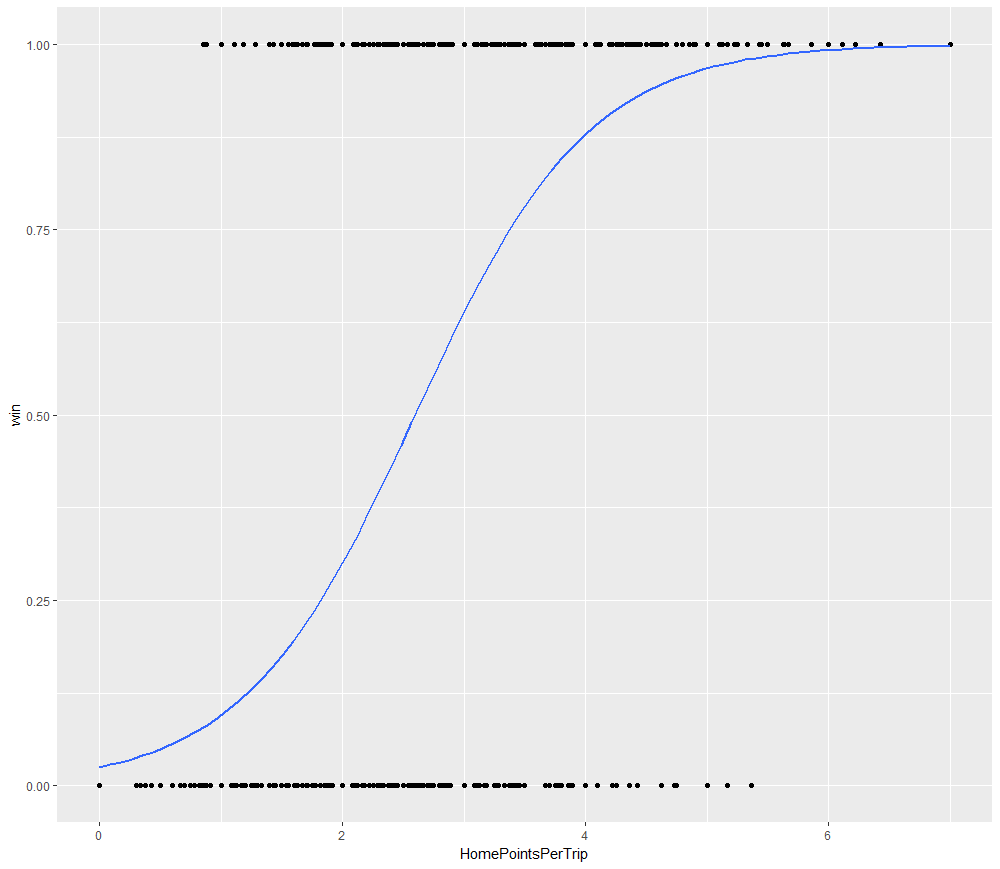
\includegraphics[scale=.5]{PPT.png}
\\
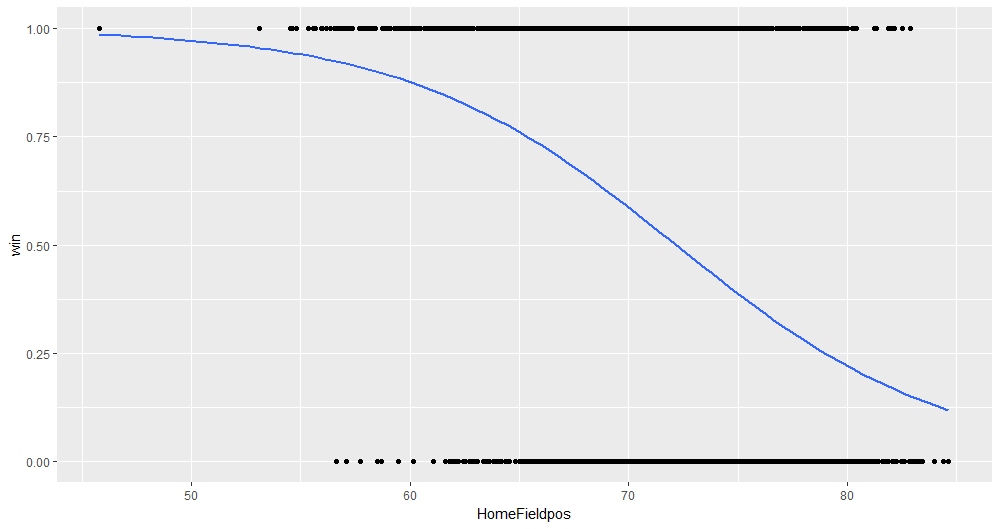
\includegraphics[scale=.5]{Field Pos.png}

\end{document}

